\section{Reconstruction of Collision Events in the ATLAS Detector}%
\label{sec:object_reco_at_atlas}

Particles produced in \pp~collision events are reconstructed from their signals
in the sub-systems of the ATLAS detector. At first, low-level objects such as
charged-particle tracks, primary vertices, and clusters of calorimeter cell
signals are reconstructed. These objects are used to reconstruct and identify
high-level objects that correspond to the signatures of particles such as
electrons, muons, \tauleptons, or quarks/gluons in the form of jets.  These
objects, often referred to as \emph{physics objects}, provide estimates of the
four-momentum and other properties of the underlying particle. The same
algorithms are used to reconstruct and identify objects in simulated
\pp~collision events and in data recorded with the detector. Differences in the
performance of the object reconstruction and selection in simulation and data
are accounted for by calibration measurements of selection efficiencies,
energy/momentum scales and resolutions. The following provides a summary of the
object reconstruction relevant for this thesis.


\subsection{Charged-Particle Tracks and Primary Vertices}%
\label{sec:tracking_and_vertexing}


The reconstruction of charged-particle trajectories is referred to as track
reconstruction or tracking. The inputs to the track reconstruction in the ID of
the ATLAS detector are \emph{space-points} from the pixel and SCT detector, and
\emph{drift-circles} from the TRT. Space-points are measurements of location in
three-dimensional space obtained by clustering the charge signals of adjacent
segments in the pixel and SCT detectors~\cite{PERF-2015-08}. Drift-circles are
measurements of distance from the anode wires of individual straw-tubes in the
TRT determined by the electron drift times in the
straw-tubes~\cite{IDET-2015-01}.

Track reconstruction employs pattern recognition techniques to select
space-points and drift-circles that are compatible with the hypothesis of a
charged particle traversing through the axial magnetic field in the
ID. Least-squares fits are performed, using selected space-points and
drift-circles, to determine the parameters characterising the
trajectory. Initially, the track parameters are given at the point of closest
approach in the transverse plane (\emph{perigee}) to the beam-spot
position~\cite{PERF-2015-08}. Five parameters, $(d_0, z_0, \phi, \theta, q/p)$,
describe the track at the perigee~\cite{Akesson:2006sh}. The transverse
(longitudinal) distance of the perigee from the beam-spot position is given by
$d_0$ ($z_0$), also referred to as the transverse (longitudinal) impact
parameter of the track. The azimuthal and polar angle of the track at the
perigee is given by $\phi$ and $\theta$, respectively. The ratio of electric
charge and momentum of the particle is given by $q / p$, which is related to the
curvature of the track. After locating the vertex of the hard interaction of
interest, tracks are often re-parameterised using this point as a reference
instead of the beam-spot position.

In the ATLAS experiment, two primary tracking algorithms are used that are
referred to as the \emph{inside-out} and \emph{outside-in}
algorithms~\cite{Cornelissen:2007vba,Salzburger:2015sgq,PERF-2015-08}. The
inside-out algorithm starts by reconstructing tracks in the pixel and SCT
detector, then extending the track using measurements in the TRT. In contrast,
the outside-in algorithm starts with the reconstruction of track segments in the
TRT, which are then combined with space-points from the pixel and SCT
detectors. The outside-in algorithm is used to improve the reconstruction
efficiency for tracks from secondary particles, such as electrons produced in
conversions of photons in the detector material, for which the inside-out
algorithm can fail to reconstruct a track. The track reconstruction algorithms
provide charged-particle tracks within the ID acceptance of $|\eta| < 2.5$ and
with $\pT > \SI{500}{\MeV}$.

Reconstructed tracks are used to determine the locations of inelastic scattering
interactions between protons in the ATLAS detector. These locations are marked
by multiple charged-particle tracks originating from the same point along the
beamline and are referred to as primary vertices (PVs).
% The vertex of the hard interaction and the associated particles can be
% identified, allowing to reject reconstructed objects originating from pile-up.
The ATLAS PV reconstruction~\cite{PERF-2015-01} finds and reconstructs PVs using
an iterative fitting procedure. It starts by reconstructing a vertex at the
location of the highest track density along the $z$-direction with respect to the
beam-spot position. An adaptive vertex fitter~\cite{Fruhwirth:2007hz} is used to
iteratively determine the vertex position while weighting reconstructed tracks
according to their compatibility with the vertex position. After the fit, tracks
that are incompatible with the fitted vertex are considered as unassociated and
the process is repeated on all unassociated tracks. After the PV reconstruction,
only PVs with two or more associated tracks are kept. The PV with the largest sum of
$\pT^2$ of associated tracks is selected as the PV of the hard
interaction. Other vertices are considered as originating from
pile-up~\cite{PERF-2015-01}.


\subsection{Topological Clustering of Calorimeter Cell Signals}

The segmentation of the calorimeters in lateral and longitudinal direction
allows for the reconstruction of the three-dimensional shape of electromagnetic
and hadronic showers. These showers typically extend over multiple cells in the
calorimeter, thus requiring the combination of several cells to reconstruct a
shower. The ATLAS experiment uses a \emph{topological calorimeter cell
  clustering algorithm}~\cite{PERF-2014-07} to combine the signals of locally
connected cells passing signal and noise thresholds, thereby suppressing noise
from the calorimeter electronics and pile-up. These clusters of calorimeter
cells, referred to as topo-clusters, are used to reconstruct electromagnetic and
hadronic showers in the calorimeters. Due to fluctuations in the shower
development and calorimeter noise, multiple topo-clusters are often required to
fully reconstruct the calorimeter response to a single particle.

The ATLAS calorimeter has a different response to electromagnetic and hadronic
showers, i.e.\ the calorimeter is \emph{non-compensating}. By default, the
energies of topo-clusters are calibrated assuming the response originates from
an electromagnetic shower (EM scale). However, the development of
electromagnetic and hadronic showers leads to differences in their shower
shapes, as previously discussed in \Cref{sec:atlas_calorimeters}. This is
exploited by the \emph{local hadronic calibration}~\cite{PERF-2014-07}, which
uses shower shape information of topo-clusters to determine their likely origin
and apply an appropriately weighted combination of calibrations for
electromagnetic and hadronic showers. The energy scale of topo-clusters after
the local hadronic calibration is referred to as the LC scale.

Topo-clusters are used as inputs for the reconstruction of higher-level physics
objects in the ATLAS detector. For example, topo-clusters at EM and LC scale are
used for the reconstruction of electrons and hadronic \taulepton decays,
respectively.


\subsection{Electrons}%
\label{sec:ele_rec}

The reconstruction of electrons (and positrons) in the ATLAS detector exploits
their characteristic signature of a charged-particle track in the ID pointing
towards a narrow cluster of energy in the electromagnetic calorimeter. The
reconstruction of electrons in the region of $|\eta| < 2.47$ and excluding the
transition regions between the barrel and end-caps, $1.37 < |\eta| < 1.52$, is
described in the following based on
Refs.~\cite{ATL-PHYS-PUB-2017-022,EGAM-2018-01}.

Electron reconstruction is seeded by topo-clusters calibrated at EM scale that
have more than \SI{50}{\percent} of their energy located in cells of the
electromagnetic calorimeter, hereafter referred to as EM topo-clusters. In
addition, EM topo-clusters are only considered if the transverse energy in the
electromagnetic part of the calorimeter, $\ET^{\text{EM}}$, exceeds
\SI{400}{\MeV}. A first attempt of geometrically matching the EM topo-cluster to
an ID track is made. If the EM topo-cluster cannot be matched to a
well-reconstructed track but has a longitudinal and lateral shower shape similar
to the signature of an electron, then a second pass of tracking is performed in
a region surrounding the cluster. The second pass allows for up to
\SI{30}{\percent} of energy loss at each intersection with detector material due
to the emission of bremsstrahlung. After an ambiguity resolution scheme in case
multiple tracks match the cluster, the cluster is required to be geometrically
matched to a single track. EM topo-clusters with matched tracks are considered
as seeds for a \emph{supercluster} reconstruction algorithm if the cluster
fulfils $\ET^{\text{EM}} > \SI{1}{\GeV}$ and the matched track passes
reconstruction quality criteria. \emph{Satellite clusters}, which are EM
topo-clusters in the vicinity of the supercluster seed, are included in the
supercluster to account for electromagnetic showers being reconstructed as
multiple topo-clusters or the formation of additional clusters from electrons
emitting bremsstrahlung. After applying initial calibrations and corrections to
a supercluster, the track matching is repeated using the supercluster barycentre
instead of the barycentre of the EM topo-cluster seed. Finally, multivariate
calibrations of the electron energy and corrections from comparisons of
reconstructed electrons in data and simulation are
applied~\cite{PERF-2017-03,EGAM-2018-01}.

Electrons that are promptly produced in the hard interaction are of interest for
most physics analyses. Other sources of reconstructed electron candidates are
quark- or gluon-initiated jets that mimic the signature of an electron, or
electrons from secondary sources such as hadron decays or photon
conversions. \emph{Identification} and \emph{isolation} requirements can be
applied to select promptly produced electrons and reject electron candidates
from other sources. Electron identification is performed using a
likelihood-based classifier exploiting variables sensitive to the shower shape,
reconstruction quality of the matched track, information about transition
radiation emission in the TRT, and spatial and momentum matching between the
track and the supercluster~\cite{EGAM-2018-01}. Furthermore, in most event
topologies little detector activity is expected in the vicinity of promptly
produced electrons. Therefore, isolation variables are defined that quantify the
activity in an area surrounding the electron candidate using reconstructed
tracks and topo-clusters in the calorimeters~\cite{EGAM-2018-01}. Selections are
applied on these isolation variables to further reject backgrounds originating
from jets and non-prompt electrons.


\subsection{Muons}%
\label{sec:muon_rec}

The reconstruction of muons in the ATLAS experiment targets the signature of a
charged particle that is able to traverse the calorimeters with only minimal
energy deposition due to ionisation. The instrumentation of the MS allows for
the reconstruction of muons up to $|\eta| < 2.7$. The following description of
muon reconstruction is based on Ref.~\cite{MUON-2018-03}.

A stand-alone reconstruction of tracks in the MS is attempted by first
reconstructing straight-line segments in individual layers of the MS. Track
candidates are constructed from multiple track segments compatible with the
trajectory of a muon produced at the IP. These candidates seed a
fit to obtain the muon trajectory and the associated track parameters. Different
reconstruction methods are employed yielding five types of reconstructed muons:
\begin{description}

\item[Combined muons] are reconstructed by matching a track in the MS to a track
  in the ID. A combined fit of the ID and MS track is performed, accounting for
  the ionisation energy loss of muons in the calorimeters, to reconstruct the
  muon trajectory. Within $2.5 < |\eta| < 2.7$ combined muons may be
  reconstructed using short segments of ID tracks instead of fully reconstructed
  tracks.

\item[Inside-out muons] are reconstructed by extending a track in the ID with
  hits in the MS. The additional hits are used for a combined fit of the muon
  trajectory in the ID and MS.
  % The inside-out strategy aims to recover cases where the stand-alone track
  % reconstruction in the MS fails to find a track.

\item[MS extrapolated muons] are reconstructed by extrapolating a stand-alone MS
  track to the beamline in cases where no matching ID track is found. The MS
  track defines the properties of the reconstructed muon. % This
  % strategy improves the reconstruction efficiency of muons in the region of
  % $2.5 < |\eta| < 2.7$, which is outside the acceptance of track
  % reconstruction in the ID.

\item[Segment-tagged muons] are reconstructed by matching an ID track to one or
  more short track segments in the MS. The muon properties are determined by the
  parameters of the ID track.

\item[Calorimeter-tagged muons] are reconstructed from ID tracks of charged
  particles with a signature in the calorimeters characteristic of a minimum
  ionising particle. The ID track is used to define the properties of
  calorimeter-tagged muons.

\end{description}
Several muon identification working points are defined using these muon types
and additional requirements on the quality of the ID and MS tracks and the
compatibility of ID and MS tracks in terms of charge and momentum. In this
thesis, the \emph{loose} and \emph{medium} working points are used, which are
summarised hereafter. Of these working points, the medium working point has the
most stringent requirements on the quality of reconstructed muons. It requires
muons to be reconstructed as combined or inside-out muons or, alternatively, MS
extrapolated muons in $2.5 < |\eta| < 2.7$ to improve the reconstruction
efficiency outside the acceptance of ID track reconstruction. The \emph{loose}
working point augments the medium working point by additionally allowing
segment- and calorimeter-tagged muons in $|\eta| < 0.1$, a region with a gap in
the MS instrumentation, and relaxing the MS track quality requirements applied
to inside-out muons. Muons passing the \emph{loose} working point are a superset
of muons passing the \emph{medium} working point.

Isolation requirements are applied to reconstructed muon candidates to
distinguish prompt from non-prompt muons. A similar approach to the one adopted
for electrons, previously discussed in \Cref{sec:ele_rec}, is used.


\subsection{Jets and $b$-tagging}%
\label{sec:jet_rec}

The production of quarks or gluons in hard scattering interactions leads to the
development of collimated sprays of particles referred to as jets. Jets are
produced as a result of the colour confinement in QCD, leading to a
fragmentation of the initial quark/gluon until the energy of the resulting
fragments is sufficiently small to bind into colourless hadrons. The primary
constituents of jets are charged/neutral hadrons and photons from hadron
decays. To reconstruct the kinematic properties of the quark/gluon that
initiated the jet, the four-momenta of all particles from the fragmentation and
hadronisation process have to be collected. This task is addressed by jet
algorithms, which combine particles, or other entities, into clusters to
reconstruct jets. In the ATLAS experiment, the anti-\kt jet clustering
algorithm~\cite{Cacciari:2008gp} is most frequently used.


\subsubsection{The Anti-\kt Jet Clustering Algorithm}

The anti-\kt jet clustering algorithm operates on collections of entities with
defined four-momenta (e.g.\ topo-clusters). Any set of one or more entities can
be viewed as a pseudo-jet with a four-momentum given by the sum of the
constituent four-momenta. Pseudo-jets are sequentially combined if they are
close according to a distance metric. The distance between pseudo-jets $i$ and
$j$ is defined by the anti-\kt algorithm as~\cite{Cacciari:2008gp}
\begin{align*}
  d_{ij} &= \min\bigl( p_{\text{T}i}^{-2}, p_{\text{T}j}^{-2} \bigr)
           \frac{ \dRy(i, j)^2 }{ R^2 } \,\text{,}
\end{align*}
where $p_{\text{T}i}$ refers to the transverse momentum of pseudo-jet $i$,
$\dRy = \sqrt{\Delta y^2 + \Delta \phi^2}$ is the distance of two pseudo-jets in
the $y\phi$-plane, with $y$ being the rapidity,\footnote{The rapidity is defined
  as
  $y = \frac{1}{2} \ln\mathopen{}\left( \frac{E + p_z}{E - p_z}
  \right)\mathclose{}$, where $E$ is then energy of a particle and $p_z$ the
  momentum component along the beamline. In the ultrarelativistic limit, the
  rapidity is equivalent to the pseudorapidity.} and $R$ is the jet-radius
parameter of the algorithm. A stopping criterion for the clustering algorithm is
provided by the distance $d_{i\text{B}} = p_{\text{T}i}^{-2}$ by proceeding as
follows~\cite{Cacciari:2008gp}:
\begin{enumerate}
\item Find the minimum distance $d_{ij}$ for all pairs of distinct pseudo-jets
  ($i \neq j$) and the minimum distance $d_{i\text{B}}$ for all pseudo-jets.

\item If $\min_{i,j}(d_{ij}) < \min_{i}(d_{i\text{B}})$: The pair of pseudo-jets
  corresponding to the minimum in $d_{ij}$ is combined to form a new pseudo-jet.

\item If $\min_{i,j}(d_{ij}) \geq \min_{i}(d_{i\text{B}})$: The pseudo-jet
  yielding the minimum $d_{i\text{B}}$ is declared as a jet and removed from the
  procedure.
\end{enumerate}
These steps are repeated until no pseudo-jets are left.

The anti-\kt algorithm produces conical jets with a typical radius of $\dRy = R$
provided no high-\pT emissions are located in the vicinity of the jet. The
algorithm has desirable theoretical properties, such as reconstructed jets being
insensitive to soft or collinear emissions~\cite{Cacciari:2008gp}, thus making
it the choice of the default jet clustering algorithm in the ATLAS
experiment. In this thesis, the jets are clustered using the anti-\kt algorithm
with a jet-radius parameter of $R = 0.4$. The implementation of the
\textsc{FastJet} library~\cite{Fastjet} is used.


\subsubsection{Jet Reconstruction using Particle Flow}

% The inputs to the jet algorithm are provided by a particle flow reconstruction
% algorithm, described in Refs.~\cite{PERF-2015-09,JETM-2018-05}, exploiting the
% superior momentum resolution of the tracking system for charged particles with
% low transverse momenta by replacing the calorimetric measurement of their
% energy with a tracking-based momentum measurement, necessitating the
% subtraction of energy deposits by charged particles in the calorimeter. The
% particle flow algorithm provides an improved jet energy and angular resolution
% as well as pile-up stability compared to jets constructed based on topological
% clusters in the calorimeters (at EM scale)
% only~\cite{PERF-2015-09,JETM-2018-05}.

Earlier analyses performed by the ATLAS collaboration used jets reconstructed by
applying the anti-\kt algorithm to topo-clusters in the calorimeters,
disregarding any information about charged particles from the tracking
system. Techniques combining information from tracking and calorimetry are now
adopted by the ATLAS experiment for the reconstruction of jets. These are based
on a reconstruction algorithm referred to as \emph{particle flow} that attempts
to reconstruct individual charged and neutral particles from their detector
signatures.
% \footnote{The idea of particle flow reconstruction dates back to collider
% experiments of the 1990s at LEP and HERA~\cite{PERF-2015-09}.}

Jet reconstruction based on particle flow, described in
Refs.~\cite{PERF-2015-09,JETM-2018-05}, exploits the superior energy and angular
resolution of reconstructing low-\pT charged hadrons from their track in the ID
instead of using calorimetric measurements.\footnote{The charged pion mass is
  assumed for the relationship between the momentum and energy of charged
  particles in the tracker.} Neutral particles have to be reconstructed from
topo-clusters in the calorimeter, making it necessary to subtract the energy
deposited by charged hadrons to prevent double-counting. This subtraction is
performed by the particle flow algorithm to reconstruct neutral particles in the
form of \emph{neutral particle flow objects}. Similarly, charged hadrons
reconstructed from their track in the ID are referred to as \emph{charged
  particle flow objects}.  Charged and neutral particle flow objects are used as
inputs to the anti-\kt jet clustering algorithm to reconstruct jets used for
physics analyses.

Jet reconstruction using particle flow has several advantages compared to a
calorimeter-based approach as detailed in Ref.~\cite{PERF-2015-09}. The energy
resolution for jets at low transverse momenta
($p_\text{T, jet} \lessapprox \SI{50}{\GeV}$, see for example
Ref.~\cite{JETM-2018-05}) is improved due to the inclusion of tracking
information. In part, this is due to the ability to account for charged hadrons
with transverse momenta down to \SI{500}{\MeV} in the reconstruction of jets. In
comparison, calorimeter-based jet reconstruction has shortcomings in accounting
for low-\pT charged hadrons due to charged hadrons being bent out of the jet
clustering cone or their calorimeter signals being suppressed by the noise
thresholds of the topo-cluster algorithm. Moreover, jets reconstructed using
particle flow are less susceptible to pile-up since charged particle flow
objects can be associated to the PV of the hard interaction.


\subsubsection{$b$-tagging}

The production of $b$-quarks is an important signature of many physics processes
at the LHC. A $b$-quark produced in a hard scattering interaction leads to the
formation of a jet, referred to as a $b$-jet. A distinct feature of $b$-jets is
the presence of a $b$-hadron with a mass exceeding \SI{5}{\GeV}~\cite{pdg2020}.
These $b$-hadrons are short-lived and decay after traversing a short but often
measurable distance in the ATLAS detector. For example, the lightest $B$-mesons,
the $B^0$ and $B^\pm$, have proper lifetimes of about
\SI{1.5e-12}{\second}~\cite{pdg2020} and thus, assuming a $B$ meson momentum of
\SI{10}{\GeV}, a mean flight path of about \SI{1}{\milli\metre} before
decaying. The dominant decay modes of $b$-hadrons produce final states
containing $c$-hadrons, which also decay after traversing a short distance in
the detector.

The task of identifying $b$-jets is referred to as $b$-tagging. Features
resulting from displaced decays of $b$- and $c$-hadrons can be exploited for
this purpose. Two categories of features are used by the $b$-tagging algorithms
employed in this thesis:
\begin{description}

\item[Track impact parameter based features] Due to the large mass of
  $b$-hadrons, the daughter particles of displaced $b$-hadron decays are
  produced at an angle with respect to the initial flight direction of the
  $b$-hadron. Consequently, the tracks of the daughter particles tend to have
  larger longitudinal and transverse track impact parameters with respect to the
  PV of the hard interaction compared to promptly produced charged
  particles. The deviation of an impact parameter from zero is quantified in
  terms of the \emph{impact parameter significance} by dividing the impact
  parameter by its uncertainty.

\item[Secondary vertex based features] Secondary vertices resulting from the
  daughter particles of $b$- and $c$-hadron decays can be reconstructed using
  charged-particle tracks measured in the ID. Among others, the displacement of
  the reconstructed secondary vertex from the PV of the hard interaction or the
  invariant mass of the charged particles associated to the vertex can be used
  as features in $b$-tagging.
\end{description}

The $b$-tagging algorithms used at the ATLAS experiment combine the
discriminants of multiple low-level algorithms. In this thesis, the
\textsc{DL1r} $b$-tagging algorithm~\cite{FTAG-2019-07} is used, which uses
neural networks to combine the outputs of the following algorithms:
\begin{description}

\item[IP2D \& IP3D] The \textsc{IP2D} and \textsc{IP3D}
  algorithms~\cite{ATL-PHYS-PUB-2017-013} provide $b$-tagging discriminants
  based on likelihood-ratio classifiers constructed from the distribution of
  impact parameter significances in $b$-, $c$-, and \emph{light}-quark
  jets. While \textsc{IP2D} only considers the distribution of the transverse
  impact parameter significance of tracks, \textsc{IP3D} considers the joint
  distribution of transverse and longitudinal impact parameter significances.
  In both cases, the likelihoods of all tracks in the jet are combined by
  neglecting any dependencies of the impact parameters between tracks.

\item[RNNIP] The \textsc{RNNIP} algorithm~\cite{ATL-PHYS-PUB-2017-003} extends
  the idea of \textsc{IP2D} and \textsc{IP3D} by also considering dependencies
  of impact parameter significances between tracks associated to a jet. This is
  accomplished with a recurrent neural network taking the tracks of a jet as
  inputs. Track properties, such as the impact parameter significances, are
  passed to the network with every track. Based on these inputs, \textsc{RNNIP}
  estimates the probability of a jet being a $b$-, $c$-, or
  \emph{light}-quark jet.

\item[SV1 \& JetFitter] The \textsc{SV1}~\cite{ATL-PHYS-PUB-2017-011} and
  \textsc{JetFitter}~\cite{ATL-PHYS-PUB-2018-025} algorithms reconstruct the
  vertices resulting from the displaced decays of $b$- and $c$-hadrons. While
  \textsc{SV1} reconstructs a single secondary vertex, \textsc{JetFitter}
  attempts to reconstruct the cascade of $b$- and $c$-hadron decays with a
  secondary and tertiary vertex. The vertices determined by both algorithms are
  used to define discriminating variables that are provided to the high-level
  $b$-tagging algorithms. Examples of these variables are the invariant mass of
  the tracks associated to the vertices or the significance of the distance
  between the secondary vertex and the PV of the hard interaction.

\end{description}
The \textsc{DL1r} $b$-tagging algorithm combines these discriminants with basic
kinematic properties of the jet to yield a high-level $b$-tagging discriminant.
Selections on this discriminant define several $b$-tagging working points with
different probabilities of correctly identifying a $b$-jet, referred to as the
$b$-tagging efficiency. In this thesis, a working point with \SI{77}{\percent}
$b$-tagging efficiency in simulated \ttbar events is used.  This working point
has $c$- and \emph{light}-quark jet rejection factors of approximately 6 and 200
in simulated \ttbar events, respectively~\cite{FTAG-2019-07}.

% Alternative source for rejection factors:
% http://atlas.web.cern.ch/Atlas/GROUPS/PHYSICS/PLOTS/FTAG-2019-005/


\subsection{Tau Leptons}%
\label{sec:tau_rec}

The \taulepton is the heaviest lepton in the SM with a mass of
\SI{1.777}{\GeV}~\cite{pdg2020}. It is sufficiently massive to decay into final
states with a charged lepton or hadrons. These decay modes are referred to as
leptonic (\taulep) and hadronic (\tauhad) decay modes, respectively. The
\taulepton decay and its branching ratios are depicted in
\Cref{fig:tau_feynman_br}. The majority of \taulepton decays produce final
states with one or three charged hadrons, predominately $\pi^{\pm}$, which are
referred to as 1- and 3-prong \tauhad, respectively.

\begin{figure}[htb]
  \begin{subfigure}[b]{0.47\textwidth}
    \centering

    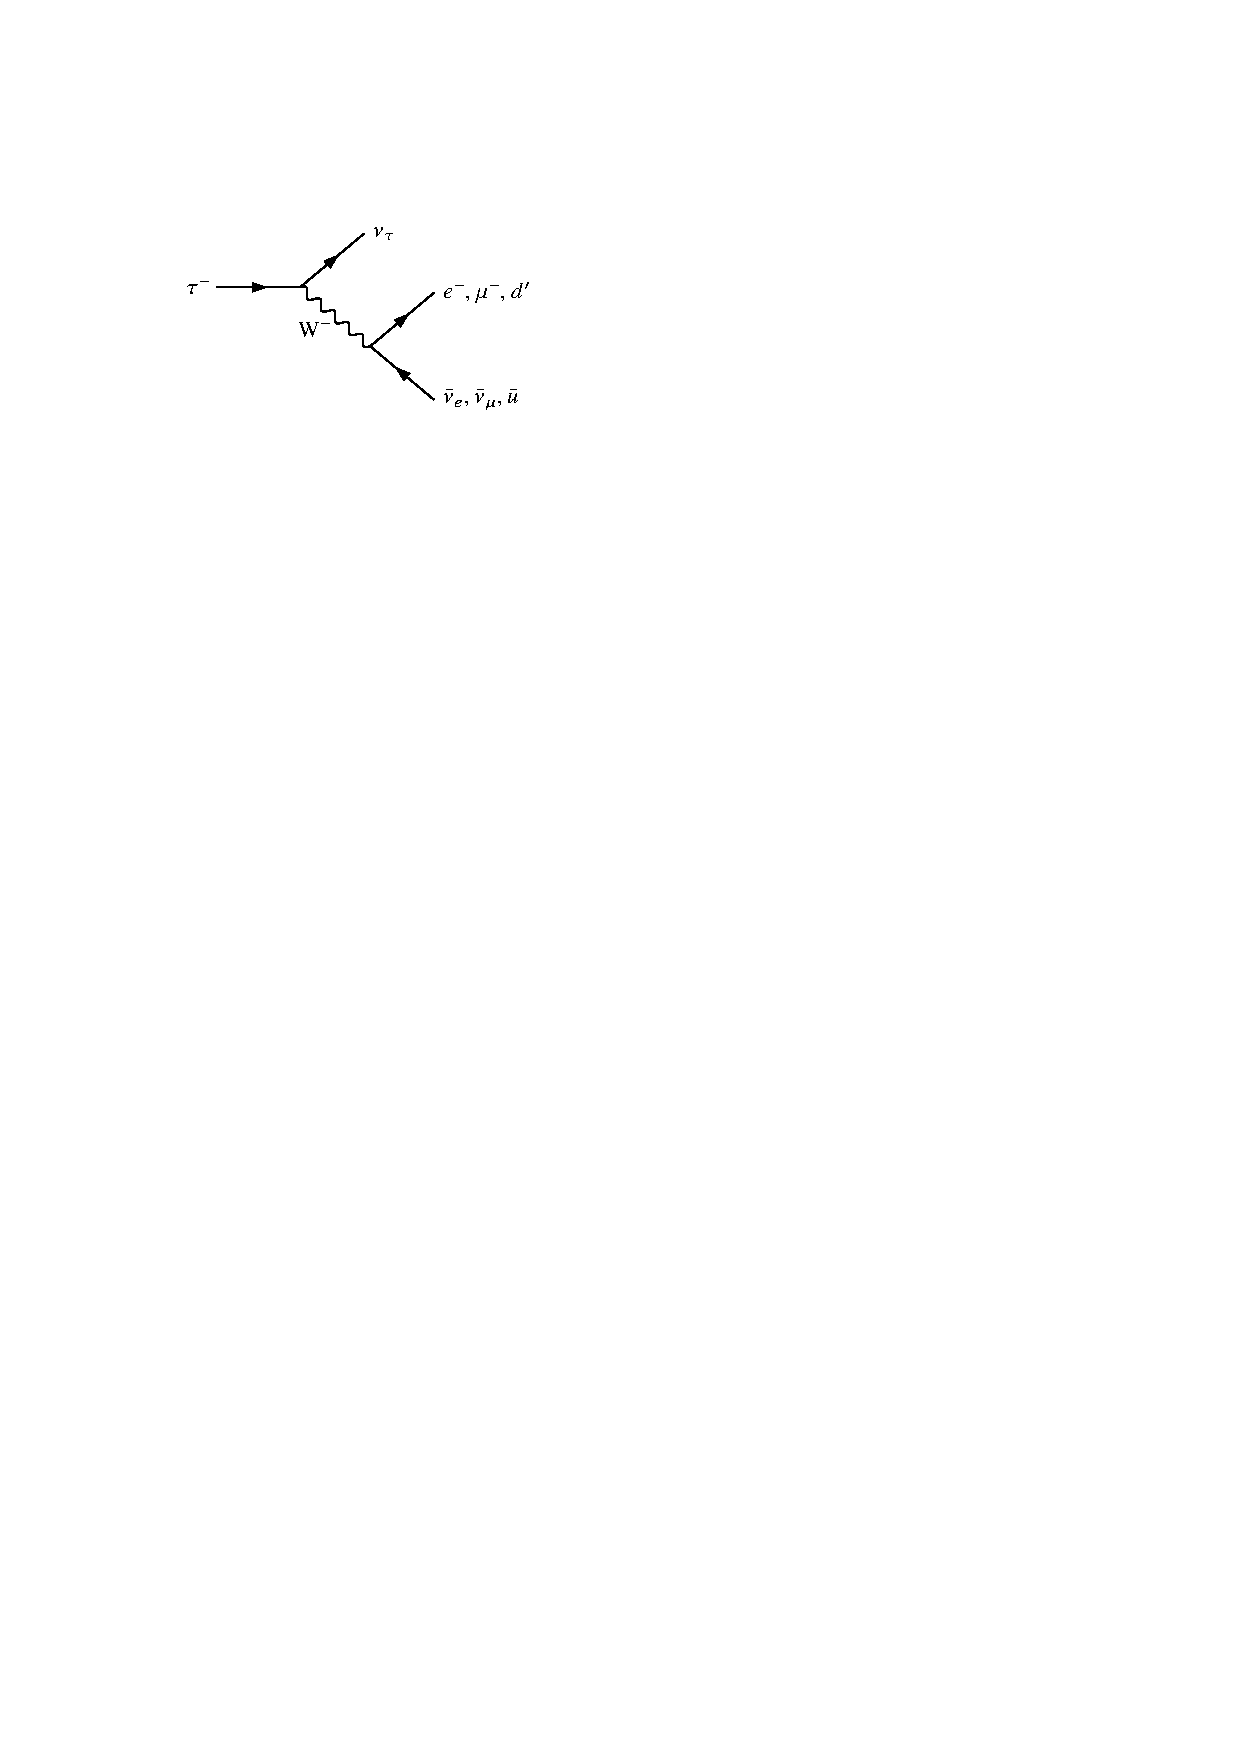
\includegraphics[width=0.75\textwidth]{figs/tauid/tau_decay_feynman}

    \vspace*{3em}
    \subcaption{}%
    \label{fig:tau_feynman}
  \end{subfigure}\hfill
  \begin{subfigure}[b]{0.47\textwidth}
    \centering

    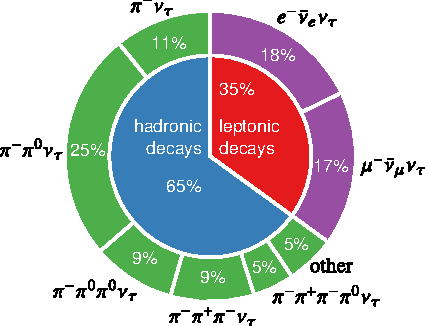
\includegraphics[width=0.85\textwidth]{figs/tauid/tau_branching_pie_chart_new}
    % \begin{overpic}[scale=0.9]{figs/tauid/tau_branching_pie_chart}
    %   \put (31, 83) {$\pi^- \nu_\tau$}
    %   \put (-5.5, 45) {$\pi^- \pi^0 \nu_\tau$}
    %   \put (16, 7) {$\pi^- 2 \pi^0 \nu_\tau$}
    %   \put (40.5, 2) {$2 \pi^- \pi^+ \nu_\tau$}
    %   \put (65, 6.5) {$2 \pi^- \pi^+ \pi^0 \nu_\tau$}
    %   \put (76.5, 15.5) {other}
    %   \put (70, 77.5) {$e^- \bar{\nu}_e \nu_\tau$}
    %   \put (88.5, 41.5) {$\mu^- \bar{\nu}_\mu \nu_\tau$}
    % \end{overpic}

    \subcaption{}%
    \label{fig:tau_branching_ratios}
  \end{subfigure}

  \caption[Feynman diagram and branching ratios of the $\tau^{-}$
  decay.]{Feynman diagram (a) and branching ratios (b) of the $\tau^{-}$ decay.
    The eigenstate coupling to the $u$-quark via the $W$ boson is denoted as
    $d^\prime$.  The \taulepton decay branching ratios are taken from
    Ref.~\cite{pdg2020} rounded to the nearest integer percentage.}%
  \label{fig:tau_feynman_br}
\end{figure}

At the ATLAS experiment, \tauleptons are reconstructed from the signature of
their visible decay products, neglecting any neutrinos produced in the
decay. Leptonic \taulepton decays are reconstructed as electrons or muons using
the reconstruction techniques previously introduced
in~\Cref{sec:ele_rec,sec:muon_rec}. The remainder of this section focuses on the
reconstruction of the visible decay products of hadronic \taulepton decays,
referred to as \tauhadvis, for which dedicated reconstruction techniques are
employed. The reconstruction of \tauhadvis at the beginning of Run~2 is
described in Ref.~\cite{ATLAS-CONF-2017-029}. Several improvements have been
made since, for example the introduction of a multivariate track selection
method~\cite{duschinger}, which are included in the following description.

% Should say something about the signature of a tau jet here
The reconstruction of \tauhadvis is seeded by jets reconstructed using the
anti-\kt algorithm with $R = 0.4$ applied to topo-clusters at LC scale. Only
jets with $\pT > \SI{10}{\GeV}$ and within $|\eta| < 2.5$ are considered as
seeds for \tauhadvis reconstruction.

A PV is associated to the \tauhadvis candidate using tracking information. The
PV association considers ID tracks that are matched to the seed jet via
ghost-association~\cite{Cacciari:2008gn}, are within $\Delta R < 0.2$ of the jet
axis, and fulfil $\pT > \SI{1}{\GeV}$ and basic track quality criteria. For
every PV, the scalar sum of \pT of tracks that are assigned to the vertex and
pass the selection criteria is determined. The PV maximising this sum is
associated to the \tauhadvis candidate and is referred to as the \emph{tau
  vertex}.

An initial estimate of the \tauhadvis candidate four-momentum is derived by
summing the four-momenta of topo-clusters (at LC scale) in a cone of
$\Delta R < 0.2$ about the jet axis. Afterwards, the four-momentum is
transformed into the coordinate system with the tau vertex at its origin. The
axis defined by the tau vertex and the three-momentum of the \tauhadvis
candidate is referred to as the \tauhadvis axis.

Tracks in the ID are associated to a \tauhadvis candidate if they are within
$\Delta R < 0.4$ of the \tauhadvis axis. Tracks originating from charged hadrons
produced in the \taulepton decay are identified by Boosted Decision
Trees~\cite{duschinger}. These tracks are referred to as \emph{core} tracks,
since they are usually found in the \emph{core region} of $\Delta R < 0.2$ about
the \tauhadvis axis. The number of \emph{core} tracks associated to a \tauhadvis
candidate is referred to as \Ntracks. Only candidates with $\Ntracks = 1$ and
$\Ntracks = 3$ are considered and referred to as 1- and 3-prong \tauhadvis
candidates, respectively. Tracks not classified as \emph{core} are classified as
\emph{isolation} tracks if they fulfil
\begin{align*}
  & \pT > \SI{1}{\GeV} && |d_{0}| < \SI{1.0}{\milli\metre} && |z_{0} \sin\theta| < \SI{1.5}{\milli\metre} \\
  & N_{\text{pixel}} \geq 2 && N_{\text{pixel}} + N_{\text{SCT}} \geq 7 \,\text{,}
\end{align*}
where the track parameters are given at the perigee with respect to the tau
vertex. The number of hits on the reconstructed track in the pixel and SCT
detector layers, counting defective sensors located on the trajectory as hits,
is given by $N_{\text{pixel}}$ and $N_{\text{SCT}}$,
respectively. \emph{Isolation} tracks are used to define variables sensitive to
the charged-particle activity in the vicinity of the \tauhadvis candidate.

Calibrations of the \tauhadvis candidate four-momentum to the \tauhadvis energy
scale (TES) are derived using simulated events containing hadronic \taulepton
decays. Two different calibration methods are used:
\begin{description}

\item[Calorimeter-based TES] The calorimeter-based TES is derived from the
  initial estimate of the \tauhadvis four-momentum from topo-clusters in the
  core region of the jet seeding the \tauhadvis. First, the expected energy
  contribution of pile-up to the \tauhadvis is subtracted. This subtraction is
  parameterised as a linear function of the number of reconstructed PVs in the
  event and in bins of \tauhadvis $|\eta|$ and \Ntracks. Afterwards, the
  detector response calibration is performed as a function of the \tauhadvis
  energy after pile-up subtraction and in bins of \tauhadvis $|\eta|$ and
  \Ntracks. The \tauhadvis transverse momentum after this calibration step is
  denoted as \pTLC.

\item[BRT-based TES] The BRT-based TES is derived from \tauhadvis energy
  calibrations performed using Boosted Regression Trees (BRT). This calibration
  uses information from \emph{Tau Particle Flow}
  reconstruction~\cite{PERF-2014-06}, which attempts to reconstruct individual
  charged and neutral hadrons produced in the \taulepton decay, as inputs. Tau
  Particle Flow provides an alternative method to reconstruct the \tauhadvis
  four-momentum with improved angular resolution, and improved energy resolution
  for \tauhadvis with transverse energies below approximately
  \SI{100}{\GeV}~\cite{PERF-2014-06}. The BRT also includes variables sensitive
  to the pile-up conditions, the shapes of showers in the calorimeter, and the
  reconstructed \taulepton decay mode. In addition, \pTLC is included as an
  input since the calorimeter-based estimate of \tauhadvis \pT is superior for
  high-\pT \tauhadvis.

\end{description}
Unless otherwise noted, the BRT-based calibration is used for the remainder of
this thesis. After calibration, the relative \tauhadvis \pT resolution ranges
from \SIrange[range-units=single]{5}{7}{\percent}~\cite{ATLAS-CONF-2017-029}.

The \tauhadvis reconstruction techniques presented thus far have limited ability
to reject \tauhadvis candidates originating from sources other than hadronic
\taulepton decays. The primary source being quark- or gluon-initiated jets and
electrons that are mis-reconstructed as \tauhadvis candidates. A separate step,
referred to as \tauid, is performed to reject \tauhadvis candidates from these
sources. A description of \tauid is given in \Cref{sec:tauid}.


\subsection{Missing Transverse Momentum}%
\label{sec:atlas_met}

The missing transverse momentum, \pTmiss, is used to reconstruct the total
transverse momentum of undetected particles produced in the hard interaction. In
the laboratory frame, the colliding partons have negligible transverse momentum
and thus it holds that
\begin{align*}
  \myvec{p}_{\text{T}}^{\text{detected}} + \myvec{p}_{\text{T}}^{\text{undetected}} = \myvec{0} \,\text{,}
\end{align*}
where $\myvec{p}_{\text{T}}^{\text{detected}}$ and
$\myvec{p}_{\text{T}}^{\text{undetected}}$ are the total transverse momenta of
the detected and undetected particles produced in the hard interaction,
respectively. Therefore, the missing transverse momentum is defined as
\begin{align*}
  \pTmiss
  \coloneqq \myvec{p}_{\text{T}}^{\text{undetected}}
  = -\myvec{p}_{\text{T}}^{\text{detected}} \,\text{.}
\end{align*}
The purpose of \pTmiss is to reconstruct the total transverse momentum of non-
or only weakly interacting particles (\emph{invisible particles}) such as
neutrinos. An object-based definition of \pTmiss from Ref.~\cite{PERF-2016-07}
is used that is defined as
\begin{align}
  \pTmiss =
  - \sum \pTvec{e}
  - \sum \pTvec{\gamma}
  - \sum \pTvec{\mu}
  - \sum \pTvec{\tauhadvis}
  - \sum \pTvec{\text{jet}}
  - \pTvec{\text{soft}}
  \,\text{,}
  \label{eq:met}
\end{align}
where the summations are over selected and calibrated electrons, photons, muons,
\tauhadvis, and jets, respectively. An additional term, \pTvec{\text{soft}}, is
introduced to account for soft radiation that is not reconstructed as part of
another object. This term is estimated by summing the transverse momenta of
tracks in the ID that are associated with the PV of the hard interaction, pass
track quality criteria, and cannot be associated with any selected electron,
photon, muon, \tauhadvis, or jet. The term $\pTvec{\text{soft}}$ is also
referred to as the \emph{track soft term}.

\Cref{eq:met} illustrates the difficulties in reconstructing the total
transverse momentum of invisible particles using \pTmiss. Any detectable object
that fails to be detected, either due to detector acceptance effects or
inefficiencies in the object reconstruction, introduces deviations from the
total transverse momentum of invisible particles. Moreover, uncertainties on
transverse momenta of all reconstructed objects accumulate in the calculation of
\pTmiss, leading to large uncertainties on \pTmiss particularly in events with
high activity.

% \item[Missing transverse momentum (\pTmiss)] is used to reconstruct
%   the total transverse momentum of (undetected) weakly-interacting
%   particles produced in the hard interaction. In this search it is
%   used to reconstruct the signatures of neutrinos produced in decays
%   of \tauleptons and semi-leptonic decays of hadrons.

%   An object-based definition of the missing transverse
%   momentum~\cite{PERF-2016-07} is adopted that uses reconstructed and
%   calibrated objects, i.e.\ electrons, muons, \tauhadvis, and jets as
%   defined previously after an ambiguity resolution step introduced
%   in~\Cref{sec:overlap_removal}, as inputs to the \pTmiss
%   reconstruction. Soft charged-particle radiation that is not part of
%   any reconstructed object is accounted for by the so-called track
%   soft term. The track soft term is defined as the vectorial sum of
%   charged-particle track $\myvec{\pT}$ over all tracks passing track
%   quality criteria that are associated to the primary vertex of the
%   hard interaction but not any reconstructed object. The object-based
%   \pTmiss is subsequently reconstructed as the negative vectorial sum
%   of transverse momenta of calibrated objects and the track soft
%   term.\todo{What \pTmissAbs working point is used?}

%   The vector of the missing transverse momentum in the transverse
%   plane is denoted as \pTmiss and its magnitude as \pTmissAbs,
%   hereafter.


%%% Local Variables:
%%% mode: latex
%%% TeX-master: "../../phd_thesis"
%%% End:
